%% -*- coding: utf-8 -*-
\documentclass[12pt,pagesize,paper=landscape,paper=192mm:108mm]{scrbook} 
%1920x1080 1280x720
\areaset[current]{192mm}{108mm}
\usepackage{calc}
\usepackage[T2A]{fontenc}
\usepackage[utf8]{inputenc}
\usepackage[english,russian]{babel}
\usepackage{microtype}
\usepackage{misccorr}
\usepackage{cmap}
%\usepackage[unicode=true]{hyperref}
\usepackage{graphicx}
\usepackage{amssymb}
\usepackage{amsmath}
%\usepackage{srcltx}
\usepackage{textcomp}
\usepackage{braket}
\usepackage{xspace}
%научные символы и смайлики \smiley \frownie
\usepackage{wasysym}
\usepackage{ccicons}
\DeclareMathOperator{\Tr}{Tr}
\DeclareMathOperator{\Texp}{Texp}
\renewcommand{\epsilon}{\varepsilon}
%перенос формул в тексте
\newcommand*{\hm}[1]{#1\nobreak\discretionary{}%
  {\hbox{$\mathsurround=0pt #1$}}{}}
\begin{document}
\begin{titlepage}
  \vspace*{-0.5em}
  \begin{center}    
    \hspace*{3em}
    \begin{minipage}[t]{3em}
      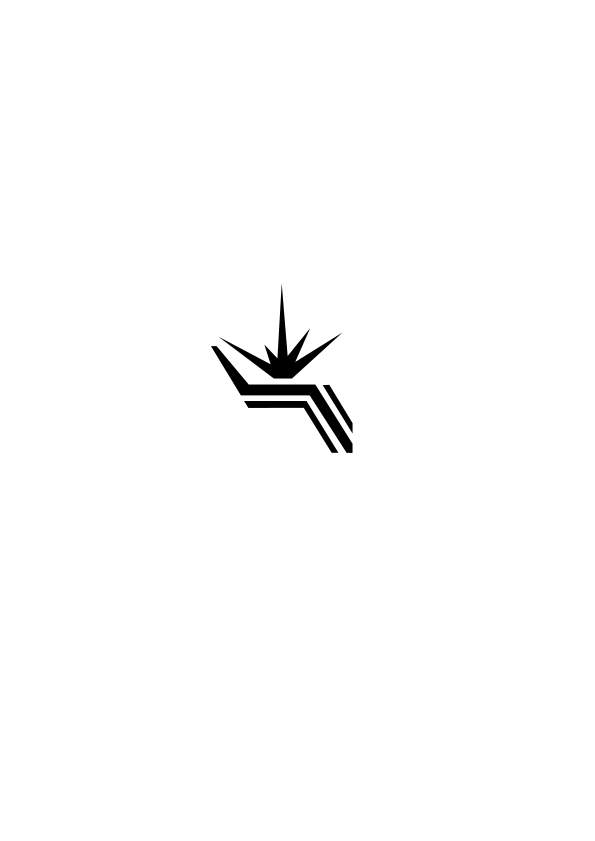
\includegraphics[width=\textwidth]{../BINP-logo}
    \end{minipage}\hfill
    \begin{minipage}{0.23\linewidth}
    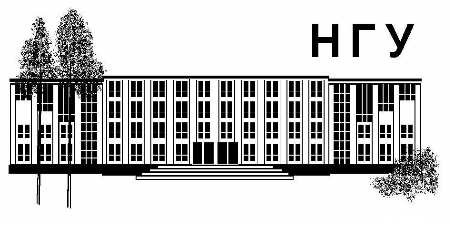
\includegraphics[width=\textwidth]{../NSU-logo}
    \end{minipage}
    \hfill
    \hspace*{6em}

    Кафедра теоретической физики физического факультета НГУ
    \medskip

    \Large
    Резниченко А.\,В.
    \bigskip

    \huge
    \textbf{Квантовая электродинамика}
    \bigskip

    \Large
    Семинар № 9
    \vfill

    \normalsize
    \vfill

    \normalsize \ccbysa\hspace{0.5em}  Новосибирск 2015
  \end{center}
\end{titlepage}
\newpage

\vspace*{-1em}
\begin{center}
\vfill
  \begin{minipage}{0.65\linewidth}
    Задача: явно проверить эрмитовость операторов в потенциале Брейта.
    \smallskip

    Задача: вычислить разницу энергий $\delta E=E({}^3S_1)-E({}^1S_0)$
    основного состояния орто- и парапозитрония.
    \smallskip

    Задача: получить часть потенциала Брейта, отвечающую
    аннигиляционной диаграмме. Формула соответствия (извлечение
    потенциала из амплитуды рассеяния). Соотношение полноты и
    соотношение Фирца для $\sigma$"=матриц Паули.

  \end{minipage}
  \vfill

  % \normalsize \ccbysa\hspace{0.5em} Новосибирск 2013
\end{center}
\end{document}
